\documentclass[tikz, border=10pt]{standalone}
\usepackage{pgfplots}
\usepackage{amsmath}
\usetikzlibrary{backgrounds}
\pgfplotsset{compat=1.18}

\begin{document}
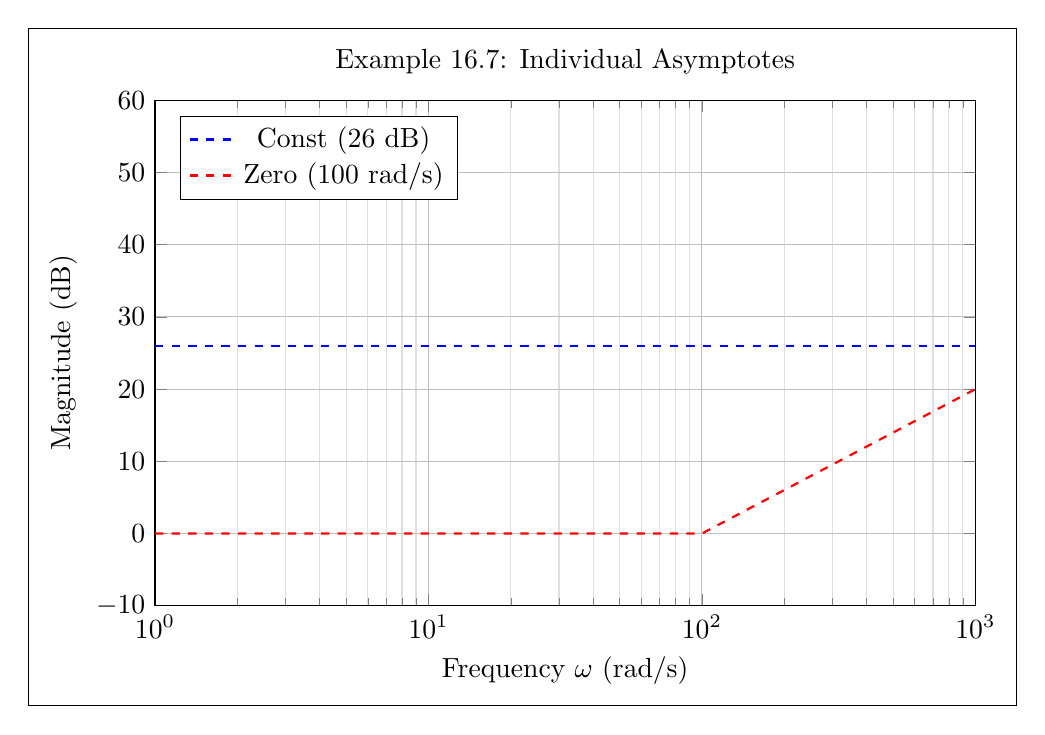
\begin{tikzpicture}[show background rectangle]
    \begin{semilogxaxis}[
        width=12cm, height=8cm,
        title={Example 16.7: Individual Asymptotes},
        xlabel={Frequency $\omega$ (rad/s)},
        ylabel={Magnitude (dB)},
        grid=both,
        xmin=1, xmax=1000,
        ymin=-10, ymax=60,
        minor grid style={gray!25},
        major grid style={gray!50},
        legend pos=north west,
    ]

    % Term 1: Constant 20 => 20log20 = 26 dB
    \addplot[blue, thick, dashed, domain=1:1000] {26};
    \addlegendentry{Const ($26$ dB)}

    % Term 2: Zero at 100 => 0 up to 100, then +20dB/dec
    % equation: 0 if x<100, 20*log10(x/100) if x>=100
    \addplot[red, thick, dashed] coordinates {
        (1, 0) (100, 0) (1000, 20)
    };
    \addlegendentry{Zero ($100$ rad/s)}
    
    \end{semilogxaxis}
\end{tikzpicture}
\end{document}
